% ICASSP 2027 submission; official spconf.sty and IEEEbib.bst.
\pdfoutput=1
\documentclass[letterpaper]{article}
\usepackage{spconf,amsmath,amssymb,graphicx}
\usepackage[T1]{fontenc}
\usepackage{booktabs,xurl,cite}
\setlength{\lightrulewidth}{0.6pt}% print stroke floor: midrule 0.5pt (0.498bp) -> 0.6pt
\usepackage[hidelinks]{hyperref}
\setcounter{topnumber}{1}
\setcounter{dbltopnumber}{1}
\setcounter{bottomnumber}{0}
\setcounter{totalnumber}{1}
\newcommand{\pos}[1]{\left[#1\right]_+}
% AUTO-GENERATED by make_tex.py from baseline_final_results.json, verify/crosslm_c5_heldout.json,
% verify/distinct_ci.json. POST HOC SECONDARY held-out analysis (not prespecified).
% Song means (mean over courses within song, then over the 80 songs); CIs are 99.5% song-bootstrap.
\newcommand{\BlPplLoopAfter}{\ensuremath{7.07}}% lm_perplexity/C4_loop_collapse: song_mean_by_dose.d3
\newcommand{\BlPplLoopPct}{\ensuremath{21}}% lm_perplexity/C4_loop_collapse: |strongest_minus_unedited_pct| (drop, %)
\newcommand{\BlPplLoopDelta}{\ensuremath{-1.85}}% lm_perplexity/C4_loop_collapse: strongest minus matched control (raw units)
\newcommand{\BlPplLoopDeltaCI}{\ensuremath{[-2.52,-1.19]}}% lm_perplexity/C4_loop_collapse: 99.5% CI of raw contrast
\newcommand{\BlPplLoopRho}{\ensuremath{+0.488}}% lm_perplexity/C4_loop_collapse: oriented rank correlation (positive = toward better)
\newcommand{\BlPplLoopRhoCI}{\ensuremath{[+0.366,+0.604]}}% lm_perplexity/C4_loop_collapse: 99.5% CI of oriented rho
\newcommand{\BlPplCommonAfter}{\ensuremath{5.89}}% lm_perplexity/C5_blandification: song_mean_by_dose.d3
\newcommand{\BlPplCommonPct}{\ensuremath{34}}% lm_perplexity/C5_blandification: |strongest_minus_unedited_pct| (drop, %)
\newcommand{\BlPplCommonDelta}{\ensuremath{-3.03}}% lm_perplexity/C5_blandification: strongest minus matched control (raw units)
\newcommand{\BlPplCommonDeltaCI}{\ensuremath{[-3.71,-2.45]}}% lm_perplexity/C5_blandification: 99.5% CI of raw contrast
\newcommand{\BlPplCommonRho}{\ensuremath{+0.759}}% lm_perplexity/C5_blandification: oriented rank correlation (positive = toward better)
\newcommand{\BlPplCommonRhoCI}{\ensuremath{[+0.700,+0.814]}}% lm_perplexity/C5_blandification: 99.5% CI of oriented rho
\newcommand{\BlPplUnedited}{\ensuremath{8.92}}% lm_perplexity: song_mean_by_dose.official
\newcommand{\BlPplCommonCrossMin}{\ensuremath{3.26}}% verify/crosslm_c5_heldout.json: min |delta_ppl_song_mean| over 3 separately fitted scorers
\newcommand{\BlPplCommonCrossMax}{\ensuremath{3.50}}% verify/crosslm_c5_heldout.json: max |delta_ppl_song_mean| over 3 separately fitted scorers
\newcommand{\BlPplCommonCrossWorstUpper}{\ensuremath{-2.64}}% verify/crosslm_c5_heldout.json: largest 99.5% upper bound of delta over 3 scorers
\newcommand{\BlSelfSimLoopAfter}{\ensuremath{0.154}}% self_similarity/C4_loop_collapse: song_mean_by_dose.d3
\newcommand{\BlSelfSimLoopPct}{\ensuremath{49}}% self_similarity/C4_loop_collapse: strongest_minus_unedited_pct (rise, %)
\newcommand{\BlSelfSimCommonAfter}{\ensuremath{0.144}}% self_similarity/C5_blandification: song_mean_by_dose.d3
\newcommand{\BlSelfSimCommonPct}{\ensuremath{40}}% self_similarity/C5_blandification: strongest_minus_unedited_pct (rise, %)
\newcommand{\BlSelfSimUnedited}{\ensuremath{0.103}}% self_similarity: song_mean_by_dose.official
\newcommand{\BlFOneFiftyJitter}{\ensuremath{1.000}}% onset_f1_50ms/C1: song mean at +-30 ms (every replicate exactly 1)
\newcommand{\BlFOneFiftyShiftSixty}{\ensuremath{0.131}}% onset_f1_50ms/C2: song mean at 60 ms shift (exactly 1 at 15, 30 ms)
\newcommand{\BlFOneTwentyJitter}{\ensuremath{0.667}}% onset_f1_20ms/C1: song mean at +-30 ms (exactly 1 at +-10, +-20 ms)
\newcommand{\BlFOneTwentyJitterDelta}{\ensuremath{-0.333}}% onset_f1_20ms/C1: strongest minus matched control
\newcommand{\BlFOneTwentyJitterDeltaCI}{\ensuremath{[-0.336,-0.331]}}% onset_f1_20ms/C1: 99.5% CI
\newcommand{\BlDistinctFourShuffleDelta}{\ensuremath{+0.21}}% verify/distinct_ci.json: distinct_4|C3 delta (rise under note-type shuffle)
\newcommand{\BlDistinctFourShuffleDeltaCI}{\ensuremath{[+0.20,+0.23]}}% verify/distinct_ci.json: distinct_4|C3 99.5% CI
\newcommand{\BlNSongs}{80}% n_songs (every cell)
% post hoc Table 2 macros (auto-generated)
\hypersetup{pdftitle={ChartGenEval: Testing Rhythm-Game Chart Measurements with Controlled Errors},
pdfauthor={Jhen-Ke Lin},pdfkeywords={Music information retrieval, rhythm games, generation evaluation, timing}}
\title{ChartGenEval: Testing Rhythm-Game Chart\\Measurements with Controlled Errors}
\name{Jhen-Ke Lin}
\address{National Yang Ming Chiao Tung University\\
\texttt{jacob.cs14@nycu.edu.tw}}
\begin{document}
\ninept
\maketitle
\suppressfloats[t]

\begin{abstract}
Evaluating rhythm-game chart generators is challenging because many
different charts can fit the same song, making reference-based comparison
inadequate and motivating the use of reference-free metrics. However, such
metrics are useful only if we understand which chart properties they
actually detect and which irrelevant changes they ignore. We introduce
ChartGenEval, a validation framework that evaluates metrics through
controlled edits to human-authored charts together with matched controls.
Using this framework on Taiko charts, we identify seven reliable metrics
spanning timing, pattern, repetition, and density, while showing that
several commonly used alternatives can overlook meaningful errors or respond
in counterintuitive ways. We further demonstrate how validated metrics can
reveal systematic issues in generated charts that conventional evaluation
may obscure. Our results suggest that chart-generation metrics should be
organized by the properties they measure and reported together with evidence
of their sensitivity and invariance.
\end{abstract}
\begin{keywords}
Music information retrieval, rhythm games, generation evaluation, timing
\end{keywords}

\begin{figure}[t]
\centering
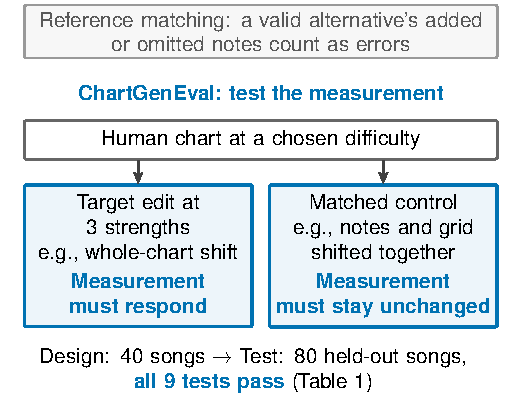
\includegraphics[width=\linewidth]{figs/overview.pdf}
\caption{ChartGenEval tests the measurement, not the chart. Reference
matching counts a valid alternative's added or omitted notes as errors. A
measurement passes when it responds to target edits of human charts and
stays unchanged under matched controls, such as a center/rim swap or notes
and grid shifted together. Controls test invariances, not acceptance of
valid alternatives. Tests are fixed on 40 development songs and
evaluated on 80 held-out songs (Table~\ref{tab:results}).}
\label{fig:overview}
\end{figure}

\begin{figure}[t]
\centering
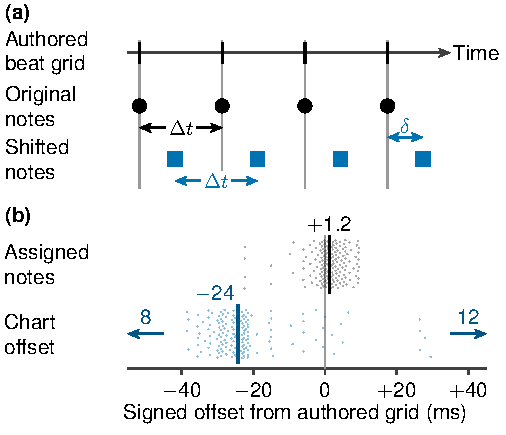
\includegraphics[width=\linewidth]{figs/timing.pdf}
\caption{A shared shift keeps note intervals but moves notes off the
authored beat grid. (a)~Shifting all notes by $\delta$ leaves each interval
$\Delta t$ unchanged; on development songs, such shifts barely change the
primary chart-only measurements, whereas chart offset recovers them
(Sec.~\ref{sec:shift}). (b)~Development songs, descriptive: in a public
generator's 170 charts (Sec.~\ref{sec:generators}), assigned notes sit
near the grid (per-chart median signed offset; median over charts
$+1.2$\,ms), whereas chart offset shows a shared shift (median $-24$\,ms; human 0\,ms).
Dots: charts; bars: medians; arrows: charts beyond the axis.}
\label{fig:timing}
\end{figure}

\section{Introduction}
\label{sec:intro}
A rhythm-game chart specifies timed player actions, such as center and rim
hits in Taiko. Chart generators map music audio to timed symbolic
events~\cite{donahue2017ddc,halina2021taikonation,
takada2023genelive,hanzen2025tcp}, much like drum transcription. Their
evaluations often match events to a
reference chart using onset-detection precision, recall, and
F1~\cite{mirevalOnset}. Unlike a transcription, however, a chart is a
design: a generated chart may legitimately add, omit, or rearrange notes for
the same song and difficulty. Matching penalizes such additions and
omissions even when both designs are suitable. It measures reconstruction,
so generation evaluation also needs measurements that reveal specific
timing, pattern, and density errors.

Reference-free statistics avoid a target chart. Music-generation studies
use distribution, diversity, and repetition
statistics~\cite{yang2020evaluation,dong2020muspy,wu2020jazz}, chart models
report perplexity~\cite{donahue2017ddc}, and human studies assess the
resulting experience~\cite{wang2024mania}. A plausible statistic can still
miss or even reward an error. A shared timing shift preserves note
intervals and types (Fig.~\ref{fig:timing}), so chart-only statistics can
miss a consistently late chart. Minimizing perplexity favors
predictability, while maximizing self-similarity favors repetition; both
can reward repetitive edits. Testing metrics with altered examples has
precedents: Fr\'echet Audio Distance is validated with artificial audio
distortions~\cite{kilgour2019fad}, Fr\'echet Music Distance with pitch and
velocity changes~\cite{retkowski2025fmd}, and SCHmUBERT presents a poor
musical example with self-similarity statistics close to its
source~\cite{plasser2023schmubert}. STRUM corrects a global offset before
scoring onset agreement~\cite{opria2026strum}.

Our key observation is that a chart measurement is interpretable only
through the errors it has been shown to detect and the changes it has been
shown to ignore. Motivated by this, ChartGenEval tests each measurement with
controlled errors (Fig.~\ref{fig:overview}). Human charts receive edits of
increasing strength, such as timing jitter, loop replacement, or burst
insertion. A measurement passes when it responds to its target edit and
stays unchanged under matched controls. We apply the
altered-example approach to chart properties with fixed controls and
held-out song tests. Timing is measured against the authored beat grid in
the song's reference chart file, which fixes musical time independently of
any chart's notes; unlike in STRUM, a chart's shared offset is a timing
error. We contribute
(i)~nine tests linking chart measurements to target edits and matched
controls, fixed on development songs before held-out evaluation;
(ii)~seven measurements of timing, pattern, repetition, and density that
pass all nine prespecified tests
on 80 held-out Taiko songs (Table~\ref{tab:results}); and
(iii)~evidence that some common statistics fail the same tests: post hoc on
held-out songs, chart-only statistics miss whole-chart shifts, and
repetitive edits lower perplexity and raise self-similarity while the
repetition score falls; on development songs, chart offset reveals an early
shift in a public generator's charts. These results support reporting the
four properties separately.

\section{Methods}
\label{sec:methods}
\subsection{Test protocol and data}
\label{sec:validation}
Each test pairs a measurement with a controlled error. Human charts receive
the target edit at three increasing strengths, and matched controls apply
changes that should leave the measurement unchanged
(Sec.~\ref{sec:edits}). For each chart, the first statistic is Spearman
correlation between output and error strength (intact plus three
strengths); the second is the strongest-edit output minus its matched
control. We reverse the signs of timing errors so expected responses to
target edits are negative for every measurement. A test passes when both
upper bounds of the 99.5\% song-bootstrap intervals lie below zero, every
control passes, and at least 72 of 80 held-out songs are evaluable. We fixed data, measurements,
edits, controls, calibration, thresholds, and analysis of these nine tests
before inspecting held-out results.

The corpus contains community-transcribed Taiko charts and associated audio.
Training uses 3{,}880 charts from 813 song groups to fit pattern models and
human comparison ranges. The held-out protocol's language model uses
trigrams and add-0.05 smoothing on the full training split.
The separate test split contains 120 song groups:
the first 40 (170 charts) were used to design measurements and edits; the
remaining 80 (333 charts) form the held-out set. Song groups merge aliases
using identifiers and audio hashes, rejecting inconsistencies. ``Song''
below refers to this grouping.

\subsection{Timing measurements}
Fig.~\ref{fig:timing} shows why timing requires information outside the
generated chart. The grid uses authored bar timestamps, meter, and
tempo from the song's reference file. This external grid fixes the time
origin independently of generated notes. Reference note times and the
generator's grid are unused. For an offset $\delta$,
\begin{equation}
 (t_{i+1}+\delta)-(t_i+\delta)=t_{i+1}-t_i,
 \label{eq:shift}
\end{equation}
so intervals alone cannot determine song alignment.

We separate note assignment from timing accuracy. Notes are matched
one-to-one to grid points by minimum-cost assignment. Assignment gates depend
on grid spacing and lie between 10 and 50\,ms. These gates decide which grid
point to compare; a tighter tolerance then scores timing. Onset-recovery
evaluations similarly allow association windows, for example 20\,ms in DDC
and 50\,ms in Gen\'eLive!~\cite{donahue2017ddc,takada2023genelive}.

For a matched note time $t_i$ and grid time $g_i$, define signed offset
$e_i=t_i-g_i$ and error beyond tolerance
\begin{equation}
 a_i=\pos{|e_i|-6\,\mathrm{ms}},\qquad [z]_+=\max(z,0).
 \label{eq:error}
\end{equation}
The 6\,ms tolerance is motivated by discrimination of a displaced tone in
short, evenly spaced sequences~\cite{friberg1995jnd}. It is an operating
choice whose perceptual validity in gameplay remains to be tested.

\textbf{On-grid fraction} is the fraction of all notes assigned within
6\,ms. Unmatched notes stay in its denominator. \textbf{Timing tail error}
is the 99th percentile of $a_i$ over a chart's matched notes. It
measures excess beyond tolerance after assignment, not raw displacement.
We also retain raw offsets and the unmatched-note fraction.

For adjacent matched notes with increasing grid times, interval distortion
is $|e_{i+1}-e_i|$. The complementary relative-error summary subtracts a
tolerance of 6\,ms or 2.5\% of the grid interval, whichever is larger, and
clips at zero, following the same study's thresholds~\cite{friberg1995jnd}.
A shared offset cancels; opposite offsets add. For example, $+4$ and
$-4$\,ms around a 200\,ms interval produce 8\,ms distortion and 2\,ms excess,
although both notes lie within the absolute tolerance. The held-out tail
test concerns $a_i$ in Eq.~\ref{eq:error}.

\subsection{Chart-offset estimation}
On a dense grid, a shifted note can match a different nearby grid point and
still receive a small local error. To estimate the shared shift, we compare
candidate offsets against fixed bar, beat, and eighth-note grids $G_k$.
Let $d(x,G_k)=\min_{g\in G_k}|x-g|$. For $n$ note times,
\begin{equation}
\begin{aligned}
 S(\delta)&=\sum_k\frac{w_k}{n}\sum_i
 \pos{1-\frac{d(t_i-\delta,G_k)}{12\,\mathrm{ms}}},\\
 \hat\delta&=\operatorname*{arg\,max}_{\delta\in[-250,250]\,\mathrm{ms}}
 S(\delta).
\end{aligned}
\label{eq:offset}
\end{equation}
Weights are 0.2, 0.3, and 0.5; the search step is 0.5\,ms.
\textbf{Chart offset} is $\hat\delta$, with $|\hat\delta|$ used in held-out
tests. Multiple grid levels reduce periodic ties, though repeated rhythms
and syncopation can leave ambiguous offsets. We test recovery for 15, 30,
and 60\,ms shifts. Tempo alone cannot fix grid phase.

\begin{table*}[t]
\centering
\caption{Held-out responses to controlled errors on 80 songs. Rank
correlation is with edit strength; strongest-edit change is the strongest
edit minus its matched control. Timing tail error and chart offset are
sign-reversed, with changes in ms, so negative values indicate the expected
response, which need not be monotone (Sec.~\ref{sec:heldout}).
Brackets show Bonferroni-adjusted 99.5\% song-bootstrap intervals. A test
passes if both upper bounds are negative, every control passes, and at least
72 songs are evaluable; all nine pass, and all 32 controls show zero
difference.}
\label{tab:results}
\setlength{\tabcolsep}{4pt}
\fontsize{9}{11}\selectfont
\renewcommand{\arraystretch}{1.15}
\begin{tabular}{@{}lllllc@{}}
\toprule
Property & Controlled error & Measurement & Rank correlation & Strongest-edit change & Pass \\
\midrule
Timing & Timing jitter & On-grid fraction & $-0.744\;[-0.815,-0.667]$ & $-0.502\;[-0.558,-0.446]$ & \checkmark \\
 & Sparse timing errors & Timing tail error (ms) & $-0.234\;[-0.344,-0.134]$ & $-0.306\;[-0.508,-0.144]$ & \checkmark \\
 & Whole-chart shift & Chart offset (ms) & $-0.916\;[-0.981,-0.826]$ & $-55.58\;[-61.43,-49.83]$ & \checkmark \\
Pattern & Note-type shuffle & Pattern familiarity & $-0.800\;[-0.856,-0.737]$ & $-0.231\;[-0.262,-0.199]$ & \checkmark \\
Repetition & Loop replacement & Repetition score & $-0.445\;[-0.573,-0.312]$ & $-0.165\;[-0.226,-0.108]$ & \checkmark \\
 & Common-pattern rewrite & Repetition score & $-0.358\;[-0.459,-0.258]$ & $-0.131\;[-0.189,-0.078]$ & \checkmark \\
 & Window shuffle & Repetition score & $-0.589\;[-0.728,-0.435]$ & $-0.224\;[-0.293,-0.156]$ & \checkmark \\
Density & Note-rate scaling & Note-rate score & $-0.693\;[-0.784,-0.579]$ & $-0.582\;[-0.672,-0.483]$ & \checkmark \\
 & Burst insertion & Density-spike score & $-0.940\;[-0.950,-0.930]$ & $-0.619\;[-0.644,-0.593]$ & \checkmark \\
\bottomrule
\end{tabular}

\end{table*}

\subsection{Pattern and density measurements}
We compare each chart with human charts at the same difficulty category
(called a \emph{course} in Taiko: Easy, Normal, Hard, Oni, or Ura). A token
encodes a note's type and quantized interval from the prior note.
\textbf{Pattern familiarity} is $\exp(-r/0.08)$, where $r$ is the fraction
of three-token sequences unseen in training at that difficulty.

For repetition and density, let $l$ and $u$ be the 10th and 90th training
percentiles and $h=\max((u-l)/2,10^{-9})$. Define
\begin{equation}
 d(x)=\frac{\max(l-x,0,x-u)}{h},\qquad s(x)=\frac{1}{1+d(x)^2}.
 \label{eq:range}
\end{equation}
The score equals one inside the middle 80\% of human values and decreases
outside it. \textbf{Repetition score} applies $s$ to $(M-U)/M$, where $M$
is the number of four-token windows and $U$ is the number of unique windows.
\textbf{Note-rate score} applies $s$ to note count divided by the time
between first and last notes.

\textbf{Density-spike score} measures large local changes separately.
It is $\exp(-b/1.5)$, where $b$ is the excess of a chart's 95th-percentile
absolute local density change above its difficulty-specific training limit, in
notes/s. Local density uses two-second windows at 0.5-second steps; the
limit is the 95th training percentile of that chart-level statistic.
Keeping the seven measurements separate prevents a high pattern score from
masking a timing error or a burst of notes.

\subsection{Controlled errors and controls}
\label{sec:edits}
Table~\ref{tab:results} pairs each edit with its target measurement. Edits
create candidate failure cases with known changes in timing, note choice,
or density. Strength measures the amount of editing; perceived severity
requires player judgments. The nine edits and their three strengths are:
\textbf{timing jitter}, perturbing all note times by up to
$\pm$10/20/30\,ms; \textbf{sparse timing errors}, shifting 0.5/1/2\% of
notes by $\pm$60\,ms; \textbf{whole-chart shift}, adding 15/30/60\,ms;
\textbf{note-type shuffle}, swapping center/rim type with probability
0.2/0.4/0.8;
\textbf{loop replacement}, replacing the first 30/60/100\% of note types with a repeated
four-note-type pattern; \textbf{common-pattern rewrite}, rewriting
30/60/100\% of positions toward more likely note types;
\textbf{note-rate scaling}, multiplying density by 0.5/1.5/2;
\textbf{burst insertion}, adding 2/4/8 clusters of 8--16 notes at
12--20 notes/s; and
\textbf{window shuffle}, selecting fixed-duration windows with probability
0.3/0.6/1 and permuting their order.

Pattern edits preserve note times. Window shuffle preserves types and
within-window offsets. Its window duration is $4\cdot60/B$ seconds for
tempo $B$ in beats/min, starting at the first note. These windows need not
coincide with authored musical bars; the test addresses reordered windows
and local transitions, not musical-form validity. Edits may affect several
measurements; the tests establish sensitivity, not exclusive detection.

Controls test identity re-evaluation, a joint one-second shift of notes and
the external time origin (grid and duration), and a center/rim type swap for
timing and density measurements. A 60\,ms whole-chart shift is the matched
control for chart-only pattern and repetition measurements and an added
control for density measurements, whose matched control is the type swap.

\subsection{Statistical analysis}
Every nonzero edit and control uses five fixed seeds. Replicates are
averaged within chart, then complete difficulty variants are averaged within
song. Songs are the statistical units, and song-level averages give the
reported estimates. Timestamp arithmetic uses integer microseconds. Each
measurement has a fixed numerical equivalence tolerance. Constant responses
receive zero correlation. For density scaling, strengths are
$[0,0.5,0.5,1]$ because halving and increasing density by half have equal
departure from the original.

We draw 10{,}000 bootstrap samples of songs and use Bonferroni-adjusted
99.5\% intervals for ten prespecified rows. The original ten rows include algebraically equivalent repetition
and variety scores for common-pattern rewriting. Both were required to
pass; Table~\ref{tab:results} displays their single effective measurement,
leaving nine distinct tests of seven measurements. A chart enters only if
all required strengths, seeds, and controls are available. Deterministic
no-op and missing cells are excluded.

\section{Results}
\label{sec:results}
\subsection{Held-out evaluation}
\label{sec:heldout}
All nine tests in Table~\ref{tab:results} meet the prespecified criteria,
and all 32 controls pass with an observed difference of zero. Each test
includes all 80 songs. Sparse timing errors retain 332 complete charts,
window shuffle retains 330, and the other tests retain 333; nineteen no-op
cells were excluded.

Two responses require careful reading. The sparse-error change is 0.306\,ms
on the original larger-is-worse scale because the timing tail error measures
excess beyond 6\,ms after grid assignment, not the injected 60\,ms
displacement. A negative rank correlation also permits a nonmonotonic
response: mean on-grid fractions under jitter are 0.996, 0.616, 0.408, and
0.495. Re-matching to other grid points may explain this rebound, whose
cause remains unresolved; the on-grid fraction detects jitter but is not a
monotonic timing loss.

Human-range calibration depends on the underlying feature. In a
predeclared secondary held-out analysis, Eq.~\ref{eq:range} applied to
language-model loss fails to identify the strongest common-pattern rewrite
(change $+0.021$, nominal 95\% interval $[-0.034,0.077]$).

\subsection{Common statistics under the same tests (post hoc)}
\label{sec:baselines}
\begin{table}[t]
\centering
\caption{Common statistics under the held-out tests on 80 songs (post hoc,
not prespecified). Columns 1--9: edits in Table~\ref{tab:results} row
order. \checkmark: passes its rule; $\circ$: unchanged at
every seed and strength; $\times$: moves toward the conventionally better
value (lower perplexity; higher self-similarity, if read as better), both
intervals excluding zero; --: unchanged by design (time-only statistic,
type-only edit).}
\label{tab:baselines}
\setlength{\tabcolsep}{3.5pt}
\fontsize{9}{11}\selectfont
% AUTO-GENERATED by tables/build_baselines.py from baselines_verdict_matrix.json (sha256 06c4afcb185bed14).
% POST HOC SECONDARY analysis, not prespecified. Columns 1-9: Timing jitter, Sparse timing errors, Whole-chart shift, Note-type shuffle, Loop replacement, Common-pattern rewrite, Window shuffle, Note-rate scaling, Burst insertion.
\begin{tabular}{@{}lccccccccc@{}}
\toprule
Statistic & 1 & 2 & 3 & 4 & 5 & 6 & 7 & 8 & 9 \\
\midrule
Perplexity & \checkmark & \checkmark & $\circ$ & \checkmark & $\times$ & $\times$ & \checkmark & \checkmark & \checkmark \\
Self-similarity & \checkmark & \checkmark & $\circ$ & \checkmark & $\times$ & $\times$ & \checkmark & \checkmark & \checkmark \\
IOI-histogram JS & \checkmark & \checkmark & $\circ$ & -- & -- & -- & \checkmark & \checkmark & \checkmark \\
Onset F1, 50\,ms & $\circ$ & \checkmark & \checkmark & -- & -- & -- & \checkmark & \checkmark & \checkmark \\
Onset F1, 20\,ms & \checkmark & \checkmark & \checkmark & -- & -- & -- & \checkmark & \checkmark & \checkmark \\
\bottomrule
\end{tabular}

\end{table}
Post hoc, five common statistics took all nine
tests (Table~\ref{tab:baselines}; seven more were also computed);
each ChartGenEval measurement got only its target test. Perplexity fell from \BlPplUnedited{} to
\BlPplLoopAfter{} under loop replacement, which is model-free,
and to \BlPplCommonAfter{} under common-pattern rewrite, selected and
scored by the same model; three separately fitted scorers fell \BlPplCommonCrossMin{}--\BlPplCommonCrossMax{} (upper bounds
${\le}\,$\BlPplCommonCrossWorstUpper{}). Self-similarity rose from
\BlSelfSimUnedited{} to \BlSelfSimLoopAfter{} and \BlSelfSimCommonAfter{},
rewarding both only if higher is read as better; distinct-4 detects
both yet rises under note-type shuffle (\BlDistinctFourShuffleDelta{}
\BlDistinctFourShuffleDeltaCI{}). Maximum-matching
50\,ms onset F1~\cite{mirevalOnset} stayed \BlFOneFiftyJitter{} at
$\pm$30\,ms jitter.

\subsection{Timing-offset recovery on development songs}
\label{sec:shift}
Shifting notes by 15, 30, or 60\,ms changes no primary chart-only
measurement by more than 0.03 human standard deviations, and with the
authored grid the chart-offset estimate moves by the injected shift to
within 3\,ms for 169 of 170 charts.

\subsection{Public generator outputs on development songs}
\label{sec:generators}
Of the public generators we ran, two output Taiko note types. We omit
TaikoNation~\cite{halina2021taikonation}, whose notes after our conversion
aligned with the authored grid near chance level.
Mapperatorinator v32~\cite{mapperatorinator} produced 170 charts for the
40 development songs (courses requested as osu!\ star ratings 2.0--7.5);
these outputs were seen during measurement design, so the readings are
descriptive. The median chart offset is $-24$\,ms (Fig.~\ref{fig:timing}b;
interquartile range
$-29$ to $-19$\,ms; human 0\,ms), for reasons we did not determine, whereas
assigned notes have a median signed offset of $+1.2$\,ms (median over charts). From
Easy to Ura, note rates are a median 2.2, 2.3, 1.9, 1.3, and 1.1 times the
paired human chart's, and median note-rate scores are 0.18, 0.11, 0.19,
1.00, and 1.00 (human 1.00); median pattern familiarity is 0.05, 0.01,
0.54, 0.76, and 0.78 (human 0.66, 0.69, 0.71, 0.81, and 0.75).

\section{Discussion}
Lower perplexity indicates easier prediction, which common-pattern
rewriting achieves by reducing note-choice diversity. Self-similarity
describes repeated material~\cite{wu2020jazz}, so its increase under loop
replacement is also consistent with what it measures. These examples expose
the ambiguity of treating either direction as improved generation
quality~\cite{theis2016note}. Human-range calibration of language-model loss
also failed to detect the rewrite, so testing the intended interpretation of
a measurement is necessary even after calibration.

Local and shared timing measurements answer different questions. The
on-grid fraction summarizes small assigned errors, the timing tail error
captures rare excesses, and chart offset estimates the shared
displacement that grid assignment can hide (Sec.~\ref{sec:generators}).

In practice, a generator evaluation can report onset F1 for reconstruction
alongside the seven measurements, placing raw offsets and the
unmatched-note fraction beside the tolerance-based timing scores.

The tested measurements are candidate rewards and constraints for
reinforcement learning toward human-like charts with fewer perceptible
errors. Tests with generator
outputs should check whether score gains preserve useful note choices, and
player studies should establish perceptual benefits.

\subsection{Limitations}
The held-out study applies fixed edit families to new songs from one Taiko
corpus. Measurements and edits were designed together on development songs,
so responses to unseen generator errors remain to be tested, and the
controls check specified invariances rather than acceptance of every valid
alternative chart. Player judgments, wrong-song pairings, and removal of
musically important notes lie outside this study. Human comparison ranges
pool broad course categories, and song-bootstrap intervals treat songs as
exchangeable without modeling shared chart authors or sources.

Timing requires a reliable external grid. Repeated rhythms can produce
multiple plausible offset estimates, and the 6\,ms tolerance awaits
validation in gameplay. Held-out results cover only the fixed tolerances,
gates, and grid weights reported here. The on-grid fraction has no reference-note recall
term, so deleting off-grid notes can raise it; it should be read with
note rate and unmatched-note fraction.

\subsection{Data and code availability}
Code, evaluation summaries, and plotting scripts are available at
\url{https://github.com/JacobLinCool/ChartGenEval}. These materials support
checking the reported summary results. End-to-end regeneration of the
frozen held-out run additionally requires its exact source snapshot and raw
records, which the release does not include. Source charts and audio are
not redistributed.

\subsection{Conclusions}
ChartGenEval links seven chart measurements to specified errors and
controls. Nine tests on 80 held-out Taiko songs establish their target
responses to edits of human charts under a fixed protocol; unseen
generator errors, timing without authored grids, acceptance of valid
alternative charts, and player judgments remain untested.
In post hoc held-out tests, perplexity and self-similarity favor repetitive
edits and chart-only statistics miss timing shifts; on development songs, a
generator's charts run early.
The evidence supports reporting timing, pattern, repetition, and density
separately, each interpreted through the errors it has been tested to
detect.

\section{Acknowledgments}
Anthropic Claude and OpenAI GPT drafted, translated, edited, and revised text in all
sections, supported discussion, and, as instructed by the author, wrote
experiment and visualization code. The author verified all outputs and is
responsible for the content.

\clearpage
\section{Compliance with Ethical Standards}
This study analyzes community-transcribed charts, associated audio, and
derived numerical records. It involved no recruited participants, player
profiles, or gameplay records. Potentially copyrighted source charts,
audio, and generated charts are not redistributed. High-volume deployment of automated generation
requires platform policy and moderation. No external funding, sponsorship,
or donated computing resources supported this study. The author declares
no conflicts of interest.
\bibliographystyle{IEEEbib}
\bibliography{references}
\end{document}
